\documentclass{article}
\usepackage[utf8]{inputenc}
\addtolength{\hoffset}{-2.25cm}
\addtolength{\textwidth}{4.5cm}
\addtolength{\voffset}{-2.5cm}
\addtolength{\textheight}{5cm}
\setlength{\parskip}{0pt}
\setlength{\parindent}{15pt}
\newcommand{\ds}{\displaystyle}

\setlength{\parindent}{0in}
\usepackage{amsmath}
\usepackage{nicematrix}
\usepackage{graphicx}
\usepackage{amssymb}

\usepackage{multicol}
\usepackage{ marvosym }
\usepackage{wasysym}
\usepackage{tikz}
%\usepackage[left=3cm,right=3cm]{geometry}
\begin{document}
\pagestyle{plain}
{\scshape } \hfill {\scshape DISCRETE STRUCTURES (CO1007) - Homework 08 - Graph} \hfill {\scshape }
 
\smallskip

\hrule

\bigskip
\textbf{\underline {\textit{Instruction:}}}
\textit{Type your answers to the following questions provided by LaTeX and submit a zipped file
(included .pdf and .tex files) to E-learning (Sakai) by group (only 4-5 members in each group). Only team
leader will submit it. One page per problem. Please use the solution template which is provided; summarize
the work of each member in percentage (\%).}

\bigskip
\begin{table}[h]
\begin{tabular}{|c|c|c|c|}
\hline
\multicolumn{4}{|c|}{\textbf{GROUP 1984 ------ MEMBER LIST}}        \\ \hline
\textbf{No.} & \textbf{Name}        & \textbf{ID} & \textbf{Role} \\ \hline
\textbf{1}   & Quach Dang Giang     & 1952044     & Leader, 30\% (of the current work)        \\ \hline
\textbf{2}   & Huynh Phuoc Thien    & 1952463     & Member, 30\%      \\ \hline
\textbf{3}   & Tran Nguyen Anh Khoa & 1911419     & Member, 40\%        \\ \hline
\end{tabular}
\end{table}
\bigskip

\textbf{The number of mandatory exercise: 5/5}  

\bigskip
\section*{Problem 1 }
\subsection*{1.1}
We have: Each person may have competed 0,1,2,3 or 4 matches. However, it is impossible that 1 person have competed 4 matches AND 1 person have competed 0 match at the same time. Thus, at any moment of the tournament there are always two players having identical number of games played
\subsection*{1.2}
Imagine the tournament is a binary tree in which the teams are the leaves, the matches are the internal vertices. With n leaves, we can create n-1 internal vertices. So, let n = 8 then we have 8 teams and 7 matches happened. Let team A always won. 2 teams create an internal vertices, so if team A always won, team A will go through 3 matches which are similar to the vertices (According to the graph) 
\begin{center}
    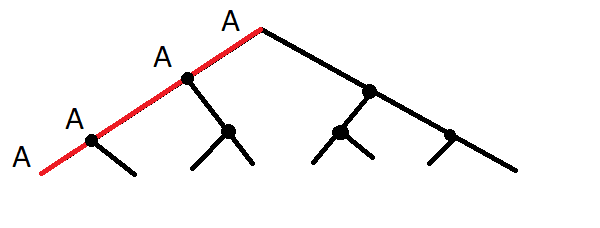
\includegraphics[scale = 0.4]{problem_1/graph1.png}
\end{center}
Thus, there exists a team that has played at least three matches if n - 1 competition games were happening.
\subsection*{1.3}
Define a graph where each vertex corresponds to a participant and where two
vertices are adjacent iff the two participants they represent know each other. Take a
vertex a of maximum degree. We claim that this vertex is adjacent to every other vertex.
Suppose, on the contrary, that there is a vertex b which is not adjacent to a. Then every
pair of vertices in the neighbourhood N(a) of a are adjacent. Furthermore, at least one of
the vertices in N(a) is adjacent to b. The degree of this vertex is larger than that of a, a
contradiction.
\subsection*{1.4}
Consider 6 people represented by dots in a circle. Let every dot be connected to every other dot by a line and let the lines be the color red if the two people know each other and blue if they do not know each other. Consider any of the 6 dots, say dot x. We can see that x is connected to 5 other dots by a line and by the pigeonhole principle 3 of these lines are the same color, say red (the proof is analogous if we choose blue instead of red) . Now examine the 3 dots connected to x. If any of those 3 people are connected by a red line, then we have found a red triangle which represents 3 people who know each other. If the 3 people are not connected by any red lines, then all 3 of them are connected by blue lines forming a blue triangle which represents 3 people not knowing each other. Thus in a group of 6 people there will always be 3 people who know each other or 3 people who do not know each other.

\subsection*{1.5}
Consider 7 people represented by dots in a circle. Let each dot connected with 3 others by a line and each line represented the letter being sent. Each dot only have 3 line connected to, so when we have connected all the lines to the dots, we have 1 dot that just has 2 lines connected to. So, there is one person who did not write back to his sender.
As we can see from the graph, the third dot just have 2 lines connected to it.
\begin{center}
    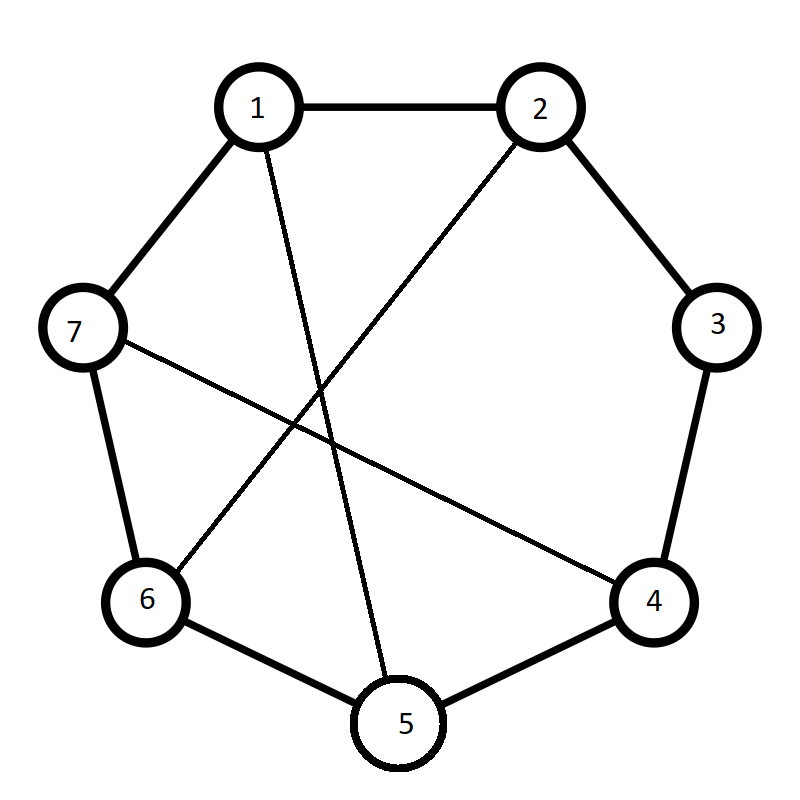
\includegraphics[scale = 0.4]{problem_1/graph2.png}
\end{center}
\bigskip
\section*{Problem 2 }
\subsection*{2.1}
\begin{table}[h]
\centering
\begin{tabular}{|c|c|c|c|c|c|}
\hline
         & $K_{n}$ & $C_{n}$ & $W_{n}$ & $K_{m, n}$ & $Q_{n}$ \\ \hline
Edges & $ \frac{n(n - 1)}{2} $ & $ n $ & $ 2n $ & $ m.n $ & $ n.2^{n - 1} $  \\ \hline
Vertices    & $ n $ & $ n $ & $ n + 1 $ & $ m + n $ & $ 2^n $  \\ \hline
\end{tabular}
\end{table}

\subsection*{2.2}
There exist simple graphs including vertices that their degree are respectively 3,3,3,3,2 and 3,2,2,1,0
\begin{figure}[h]
    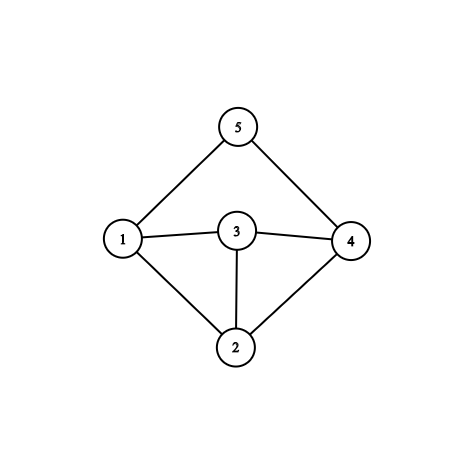
\includegraphics[scale = 0.4]{problem_2/graph_2.2.1.png}
    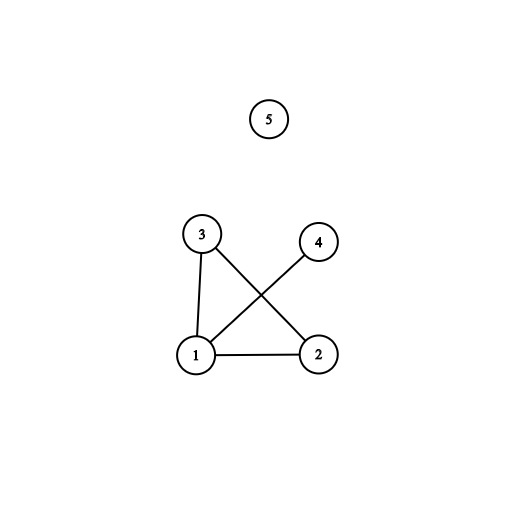
\includegraphics[scale = 0.4]{problem_2/graph_2.2.2.png}
\end{figure}
\newpage

{\scshape } \hfill {\scshape DISCRETE STRUCTURES (CO1007) - Homework 08 - Graph} \hfill {\scshape }
 
\smallskip

\hrule

\bigskip

\bigskip 
\subsection*{2.3}
There are 7 edges in a graph which has vertices of degree 4,3,3,2,2
\begin{figure}[h]
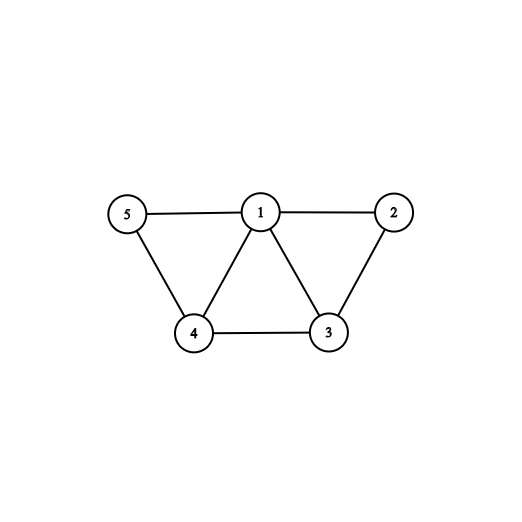
\includegraphics[scale = 0.4]{problem_2/graph_2.3.png}
\end{figure}

\subsection*{2.4}
The number of edges of $\overline{G}$ is the number of edges of the complete graph based on the number of G vertices minus the number of G edges
$$ \Rightarrow \overline{e} = \frac{v(v - 1)}{2} - e $$

\subsection*{2.5}
Apply equation from 2.4 that we have proved
$$ \overline{e} = \frac{v(v - 1)}{2} - e \Rightarrow 13 = \frac{v(v - 1)}{2} - 15 \Rightarrow v = 8 $$
$ \Rightarrow $ G has 8 vertices
\newpage

{\scshape } \hfill {\scshape DISCRETE STRUCTURES (CO1007) - Homework 08 - Graph} \hfill {\scshape }
 
\smallskip

\hrule

\bigskip

\bigskip 
\section*{Problem 3}

\subsection*{3.1}
\subsection*{Matrix 1:}
\begin{table}[h]
\begin{tabular}{c|c c c c}

  & a & b & c & d \\ \hline
a & 0 & 1 & 1 & 1 \\
b & 1 & 0 & 0 & 1 \\
c & 1 & 0 & 0 & 1 \\
d & 1 & 1 & 1 & 0 \\
\end{tabular}
\hspace{6em}
\begin{tabular}{c|c c c c c}

  & $e_{1}$ & $e_{2}$ & $e_{3}$ & $e_{4}$ & $e_{5}$ \\ \hline
a & 1 & 0 & 0 & 1 & 1 \\
b & 1 & 1 & 0 & 0 & 0 \\
c & 0 & 0 & 1 & 1 & 0 \\
d & 0 & 1 & 1 & 0 & 1 \\
\end{tabular}
\end{table}

\subsection*{Matrix 2:}
\begin{table}[h]
\begin{tabular}{c|c c c c}

  & a & b & c & d \\ \hline
a & 0 & 0 & 1 & 1 \\
b & 0 & 0 & 1 & 2 \\
c & 1 & 1 & 0 & 1 \\
d & 0 & 2 & 1 & 0 \\
\end{tabular}
\hspace{6em}
\begin{tabular}{c|c c c c c}

  & $e_{1}$ & $e_{2}$ & $e_{3}$ & $e_{4}$ & $e_{5}$ \\ \hline
a & 1 & 0 & 0 & 0 & 0 \\
b & 0 & 0 & 1 & 1 & 1 \\
c & 1 & 1 & 0 & 0 & 1 \\
d & 0 & 1 & 1 & 1 & 0 \\
\end{tabular}
\end{table}

\subsection*{Matrix 3:}
\begin{table}[h]
\begin{tabular}{c|c c c c}

  & a & b & c & d \\ \hline
a & 1 & 1 & 1 & 1 \\
b & 0 & 0 & 0 & 1 \\
c & 1 & 1 & 0 & 0 \\
d & 0 & 1 & 1 & 1 \\
\end{tabular}
\hspace{6em}
\begin{tabular}{c|c c c c c c c c c c}

  & $e_{1}$ & $e_{2}$ & $e_{3}$ & $e_{4}$ & $e_{5}$ & $e_{6}$ & $e_{7}$ & $e_{8}$ & $e_{9}$ & $e_{10}$ \\ \hline
a & -1 & 0 & 0 & 0 & 1 & -1 & 0 & 0 & -1 & 0 \\
b & 1 & 1 & -1 & 0 & 0 & 0 & 0 & 0 & 0 & -1 \\
c & 0 & 0 & 0 & 1 & -1 & 1 & 0 & 0 & 0 & 1 \\
d & 0 & -1 & 1 & -1 & 0 & 0 & 0 & 0 & 1 & 0 \\
\end{tabular}
\end{table}

\subsection*{3.2}
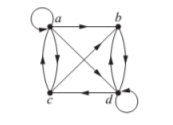
\includegraphics[scale = 2]{problem_3/graph_3.2.1.png}
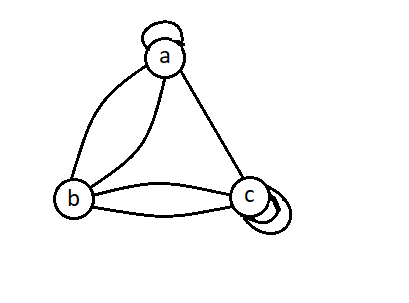
\includegraphics[]{problem_3/graph_3.2.2.png}
\newpage

{\scshape } \hfill {\scshape DISCRETE STRUCTURES (CO1007) - Homework 08 - Graph} \hfill {\scshape }
 
\smallskip

\hrule

\bigskip

\bigskip 
\subsection*{3.3}
Using Handshaking Theorem a v vertices and e edges graph, since the degree of any vertex of the graph is greater of equal than m, we have:
$$ 2e = \sum_{vertex \in V}deg(vertex) = deg(vertex_1) + deg(vertex_2) +...+ deg(vertex_v) \geqslant m.v $$
$$ \Rightarrow \frac{2e}{v} \geqslant m $$
Proving similarly, we also have:
$$ \frac{2e}{v} \leqslant M $$
Then
$$ m \leqslant \frac{2e}{v} \leqslant M $$
\newpage

{\scshape } \hfill {\scshape DISCRETE STRUCTURES (CO1007) - Homework 08 - Graph} \hfill {\scshape }
 
\smallskip

\hrule

\bigskip

\bigskip 
\section*{Problem 4}
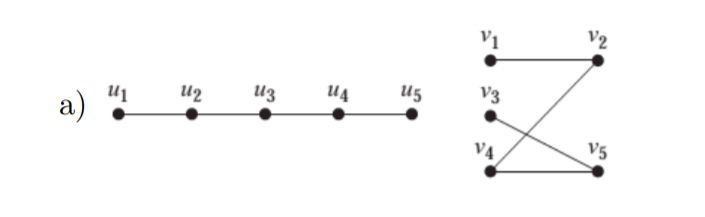
\includegraphics[scale = 0.8]{problem_4/graph_4.a.png}
\newline
The two graph are isomorphic. Isomorphism function $ f : U \rightarrow V $ with
$$ f(u_1) = v_1, f(u_2) = v_2, f(u_3) = v_4, f(u_4) = v_5, f(u_5) = v_3 $$

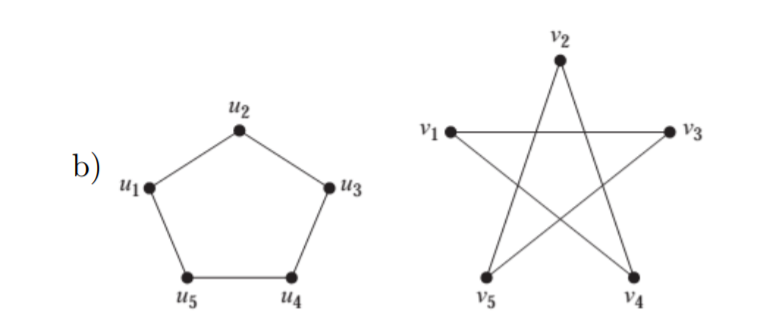
\includegraphics[scale = 0.8]{problem_4/graph_4.b.png}
\newline
The two graph are isomorphic. Isomorphism function $ f : U \rightarrow V $ with
$$ f(u_1) = v_1, f(u_2) = v_3, f(u_3) = v_5, f(u_4) = v_2, f(u_5) = v_4 $$

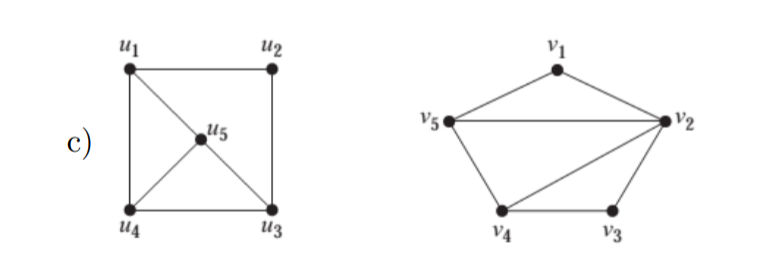
\includegraphics[scale = 0.8]{problem_4/graph_4.c.png}
\newline
The two graph are not isomorphic because the degree of $v_2$ is 4 but no vertex in the first graph has degree of 4
\newpage

{\scshape } \hfill {\scshape DISCRETE STRUCTURES (CO1007) - Homework 08 - Graph} \hfill {\scshape }
 
\smallskip

\hrule

\bigskip

\bigskip 
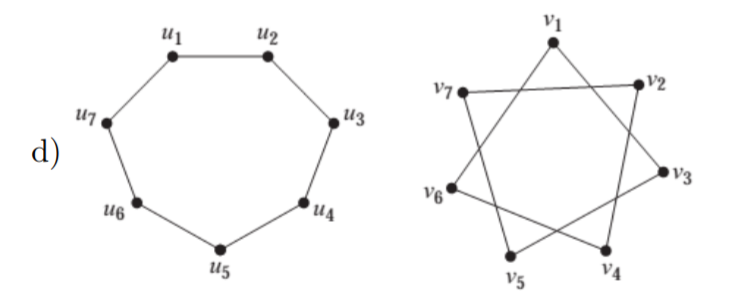
\includegraphics[scale = 0.8]{problem_4/graph_4.d.png}
\newline
The two graph are isomorphic. Isomorphism function $ f : U \rightarrow V $ with
$$ f(u_1) = v_1, f(u_2) = v_3, f(u_3) = v_5, f(u_4) = v_7, f(u_5) = v_2, f(u_6) = v_4, f(u_7) = v_6 $$

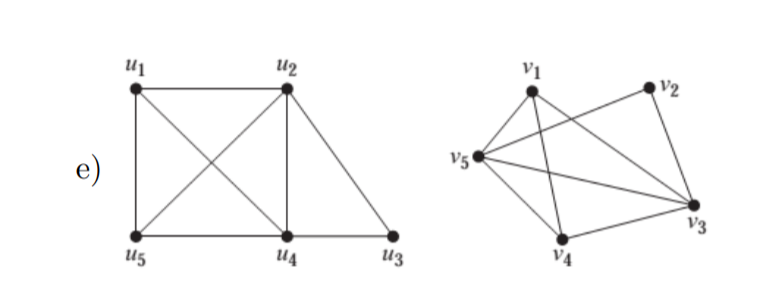
\includegraphics[scale = 0.8]{problem_4/graph_4.e.png}
\newline
The two graph are isomorphic. Isomorphism function $ f : U \rightarrow V $ with
$$ f(u_1) = v_1, f(u_2) = v_3, f(u_3) = v_2, f(u_4) = v_5, f(u_5) = v_4 $$

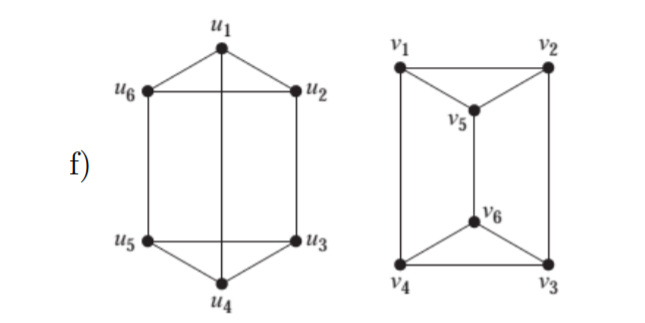
\includegraphics[scale = 0.8]{problem_4/graph_4.f.png}
\newline
The two graph are isomorphic. Isomorphism function $ f : U \rightarrow V $ with
$$ f(u_1) = v_5, f(u_2) = v_2, f(u_3) = v_3, f(u_4) = v_6, f(u_5) = v_4, f(u_6) = v_1 $$
\newpage

{\scshape } \hfill {\scshape DISCRETE STRUCTURES (CO1007) - Homework 08 - Graph} \hfill {\scshape }
 
\smallskip

\hrule

\bigskip

\bigskip 
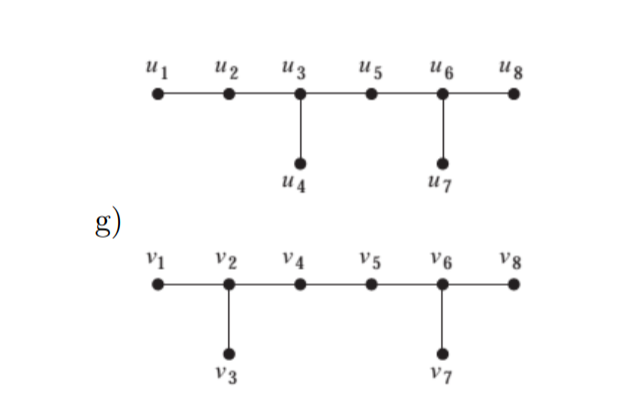
\includegraphics[scale = 0.8]{problem_4/graph_4.g.png}
\newline
The two graph are not isomorphic since their traversal path are different to each other

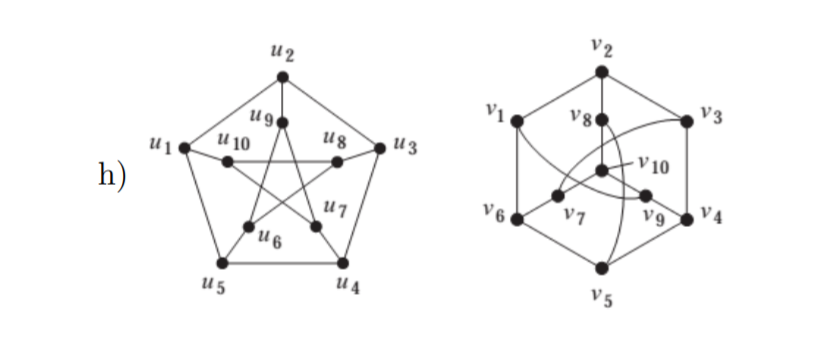
\includegraphics[scale = 0.7]{problem_4/graph_4.h.png}
\newline
The two graph are isomorphic. Isomorphism function $ f : U \rightarrow V $ with
$$ f(u_1) = v_1, f(u_2) = v_2, f(u_3) = v_3, f(u_4) = v_7, f(u_5) = v_6, f(u_6) = v_5, f(u_7) = v_{10}, f(u_8) = v_4, f(u_9) = v_2, f(u_{10}) = v_9 $$

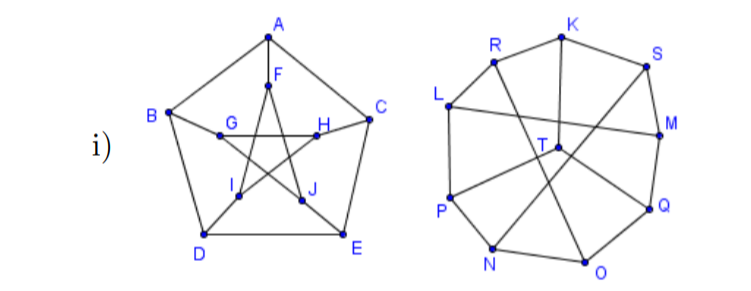
\includegraphics[scale = 0.8]{problem_4/graph_4.i.png}

The two graph are isomorphic. Isomorphism function $ f : U \rightarrow V $ with
$$ f(A) = K, f(B) = R, f(C) = S, f(D) = L, f(E) = M, f(F) = T, f(I) = P, f(J) = Q, $$
$$ f(H) = N, f(G) = O $$
\newpage

{\scshape } \hfill {\scshape DISCRETE STRUCTURES (CO1007) - Homework 08 - Graph} \hfill {\scshape }
 
\smallskip

\hrule

\bigskip

\bigskip 
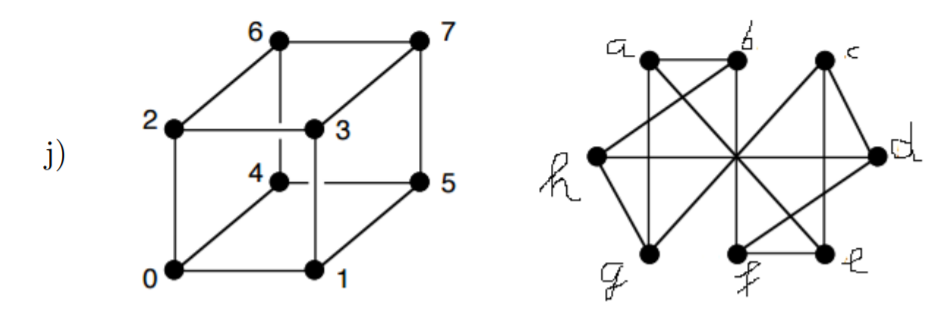
\includegraphics[scale = 0.7]{problem_4/graph_4.j.png}
\newline
The two graph are isomorphic. Isomorphism function $ f : U \rightarrow V $ with
$$ f(a) = 0, f(b) = 1, f(c) = 6, f(d) = 7, f(e) = 4, f(f) = 5, f(g) = 2, f(h) = 3 $$

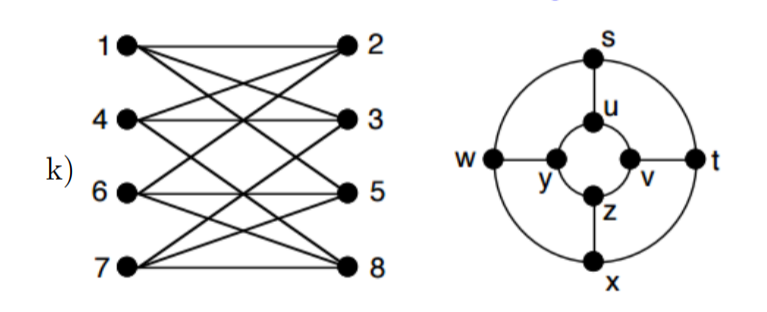
\includegraphics[scale = 0.8]{problem_4/graph_4.k.png}
\newline
The two graph are isomorphic. Isomorphism function $ f : U \rightarrow V $ with
$$ f(1) = s, f(2) = w, f(3) = t, f(4) = x, f(5) = u, f(6) = y, f(7) = v, f(8) = z $$

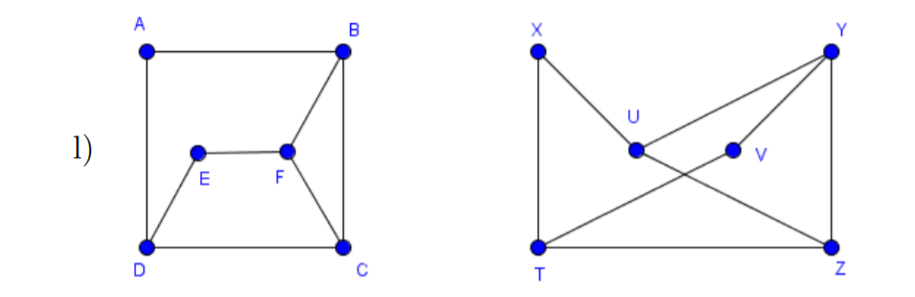
\includegraphics[scale = 0.7]{problem_4/graph_4.l.png}
\newline
The two graph are isomorphic. Isomorphism function $ f : U \rightarrow V $ with
$$ f(A) = V, f(B) = Y, f(C) = Z, f(D) = T, f(E) = X, f(F) = U $$

\end{document}
